\subsection{Post-starburst (PSB) Galaxies}
\label{sec:PSBs}
Vivienne has been involved in the preparation of a number of papers researching PSBs: \citet{2017MNRAS.472.1401A} regarding the relationship between quenching of star formation and morphological transition, while \citet{2016MNRAS.463..832W} sets out the background work.
\par Galaxy evolution has been explained by referring to a galaxy colour-magnitude diagram (CMD) as illustrated in Fig.~\ref{fig:CMD1}.

\begin{figure}
	% Allowable file formats are eps or ps if compiling using latex or pdf, png, jpg if compiling using pdflatex
	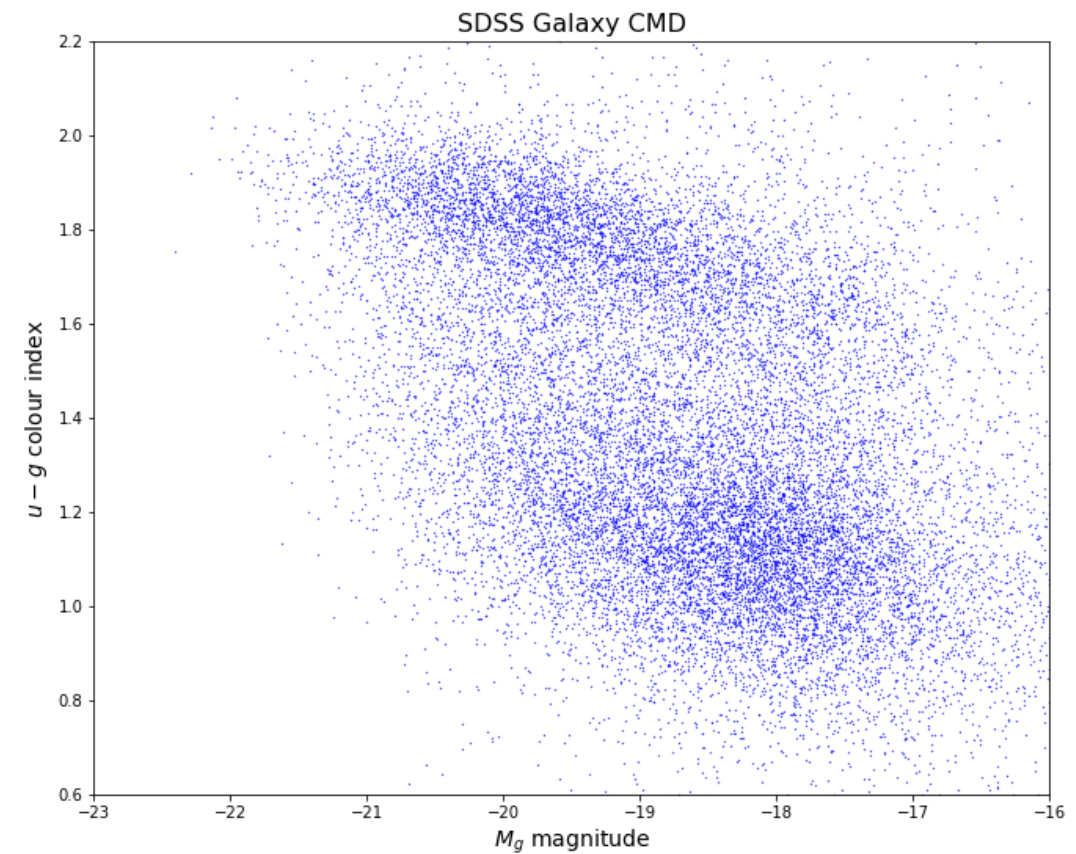
\includegraphics[width=\columnwidth]{images/galaxyCMD.PNG}
    \caption{Galaxy colour-magnitude diagram: $u-g$ colour index versus $M_g$ magnitude. The bimodality of the distribution is discussed in the text.}
    \label{fig:CMD1}
\end{figure}